\documentclass{article}

\usepackage{subcaption}
\usepackage{graphicx}
\usepackage[english]{babel}
\usepackage{listings}

\usepackage{float}
\usepackage{lipsum}
\usepackage{mwe}

\lstset{ 
  frame=single,	                   % adds a frame around the code
  numbers=left
}

\title{Abterra I}
\author{Thomas van Maaren}

\newcommand{\Website}{[placeholder]}
\newcommand{\adder}{https://www.youtube.com/watch?v=qZauC0OicRM} 
\newcommand{\BinaryWebsite}{[placeholder]}
\newcommand{\assembler}{[placeholder]}
\newcommand{\PyHow}{https://www.wikihow.com/Use-Windows-Command-Prompt-to-Run-a-Python-File}
\newcommand{\LogComp}{[placeholder]}
\newcommand{\BennysRAM}{[placeholder]}

\begin{document}
\maketitle

\begin{figure}
	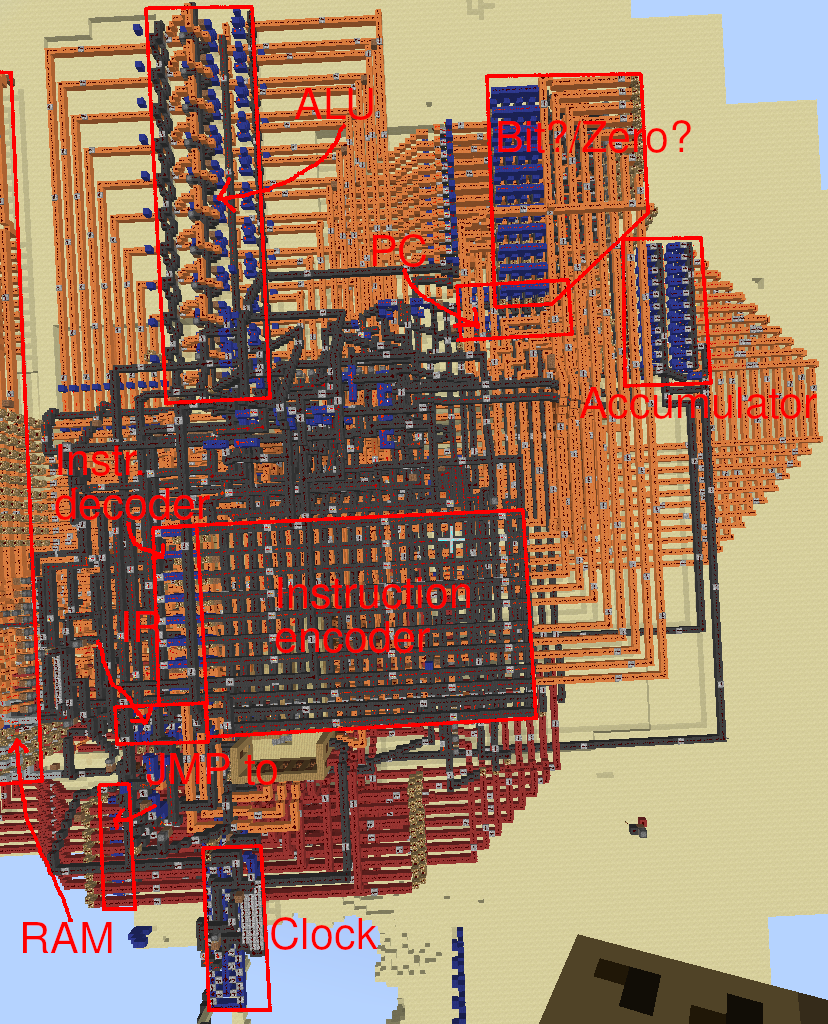
\includegraphics[width=\textwidth]{map.png}
	\caption{Map of Abterra I}
\end{figure}
\section{Introduction}
The Abterra I is a computer built in minecraft without the use of any command blocks or mods. The computer can be downloaded here: \Website. This manual shall explain the inner workings of this machine, so you will be able to program or modify it. I would advise you to learn binary and the logical operations before you read this article. This is a good source: \BinaryWebsite. It is also advisable to have some expierence in writing programs.

~\\
Maybe you are confused why this would count as a computer, because it does not fit in the stereotypical image of a computer. It does not have a keyboard or a screen for example. What you don't understand is that a screen or a keyboard are just ways for the computer to communicate with the user and are not essential to run a program.

~\\
This computer differs from other minecraft computers in a few ways:
\begin{itemize}
	\item Small and simple instruction set.
	\item Instructions and data stored in the same place.
	\item Programs can be written from the Control room.
\end{itemize}
~\\
It being a minecraft computer you shouldn't expect it to run too complex software. Here are the specs:
\begin{itemize}
	\item 256 addresses of ram, which in this case is 2816 bits
	\item 8 instructions
	\item Cpu of 48 milliherz
	\item Two clock cycles per instruction
\end{itemize}
~\\
This computer is eaven way slower than computers from the 1940's and can't really be used for any practical applications.
\section{RAM}
RAM stands for Random Access Memory. It is the place where data is stored. What is special about this minecraft computer is that the program that the computer is currently running is in the same place as the data that the program uses. a downside of this is that the computer is bigger, because the RAM has to be big enough to store a reasonably big program. The advantages of having the data and program in the same place is that the program can change itself. See section \ref{Round}. It also features an alternative way of writing the code into the computer. See section \ref{Loading in}.
\begin{figure}[H]
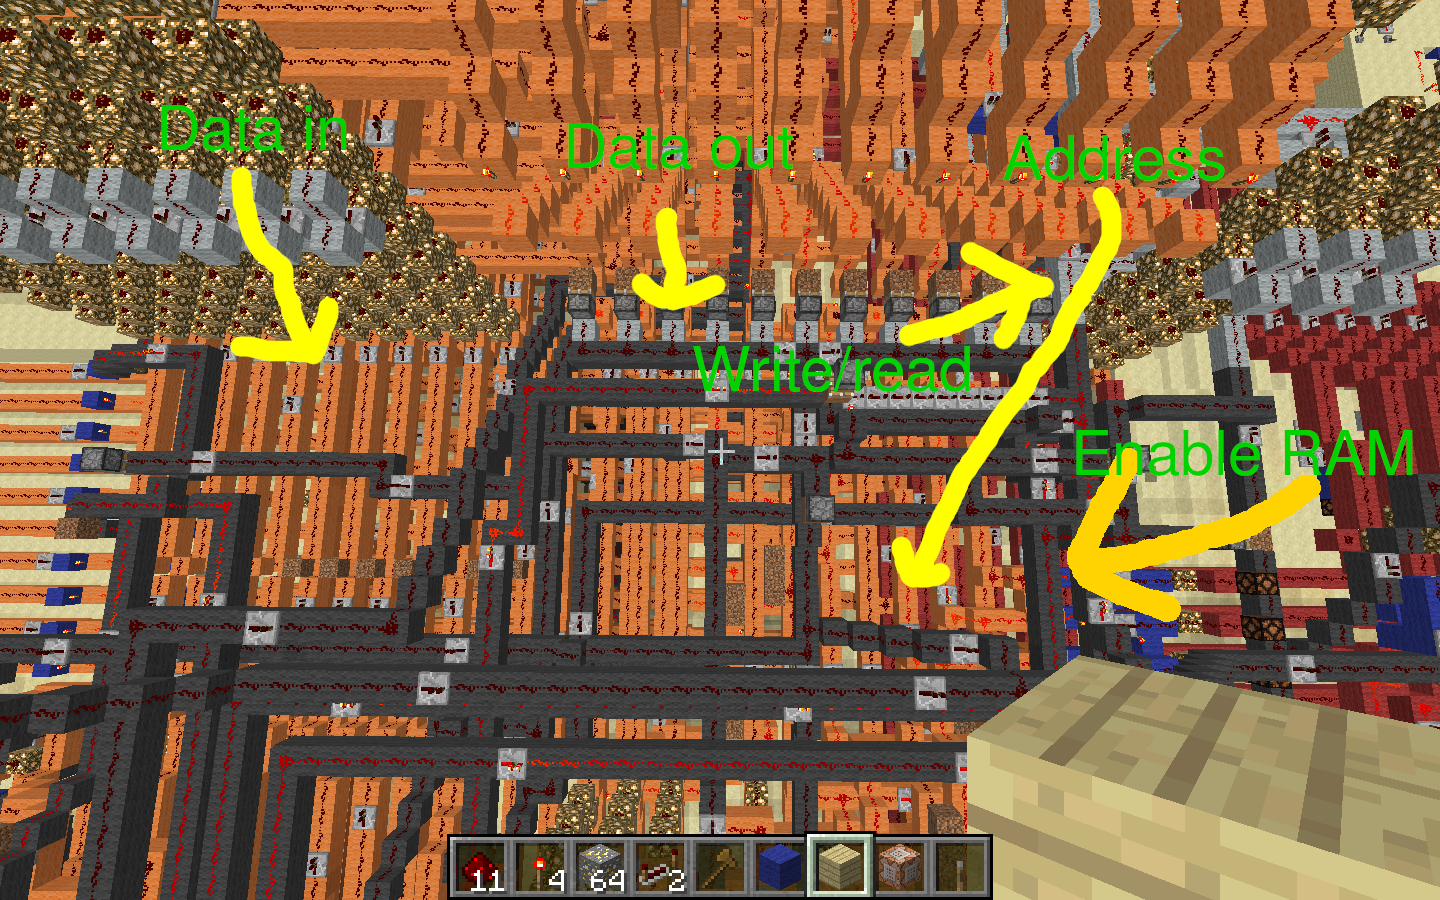
\includegraphics[width=\textwidth]{Ram in and out.png}\caption{Shows the bussses going into RAM}
\end{figure}
~\\
The RAM is comprised of 256 addresses which can be individually read or be written too by the CPU. To select which address it wants to read or write the CPU uses the address bus. This bus has eight bits which makes it capable to address all the 256 addresses. The RAM is enabled when the ``Enable RAM'' line is turned on. If it is enabled the contents of the specified address will then be put on the data out bus and if read/write is turned off and RAM is enabled the value on the ``data in'' bus shall be stored in the specified address.
\begin{figure}[h]
    \centering
    \begin{minipage}{0.5\textwidth}
        \centering
        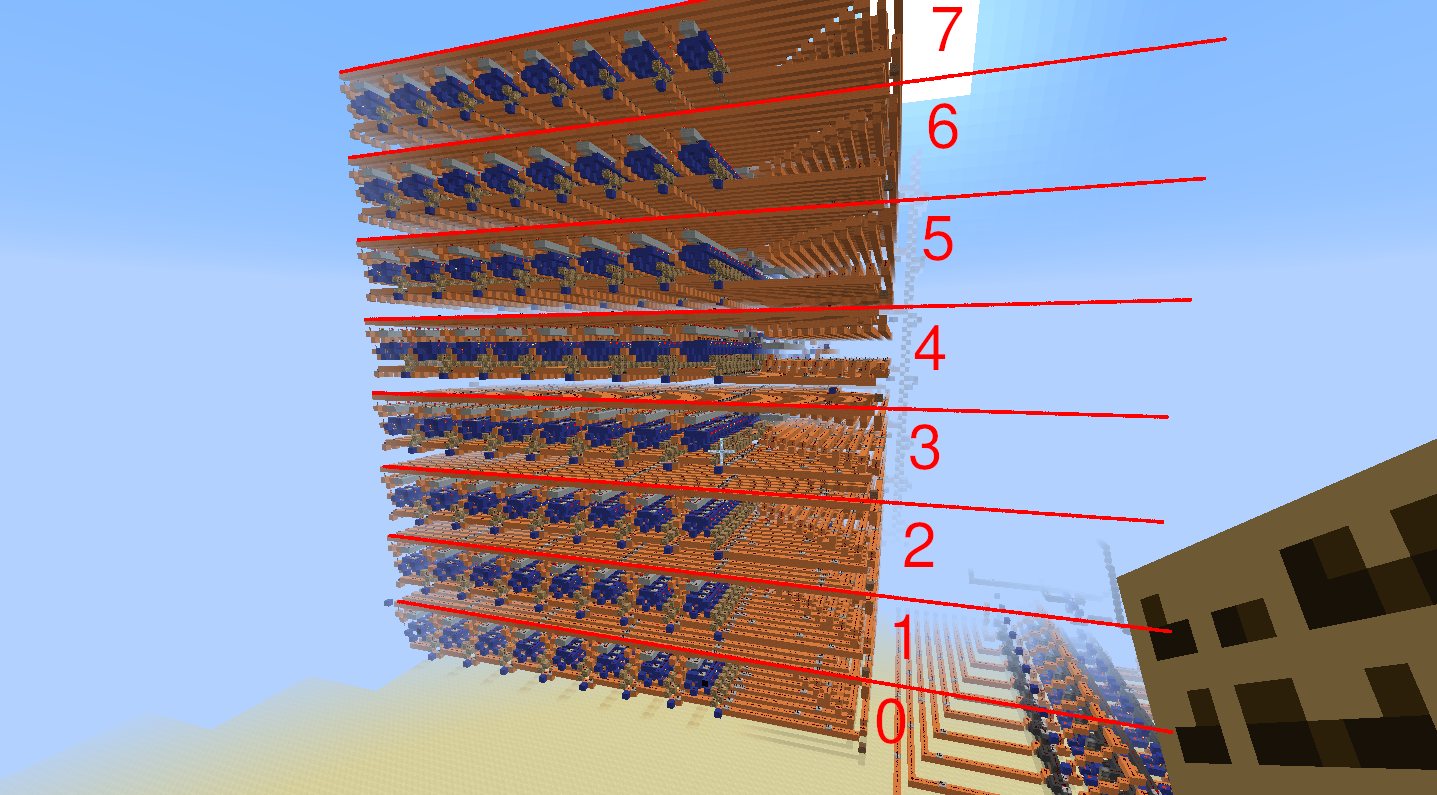
\includegraphics[width=0.9\textwidth]{Ram layers.png}
        \caption{8 layers}
    \end{minipage}\hfill
    \begin{minipage}{0.5\textwidth}
        \centering
        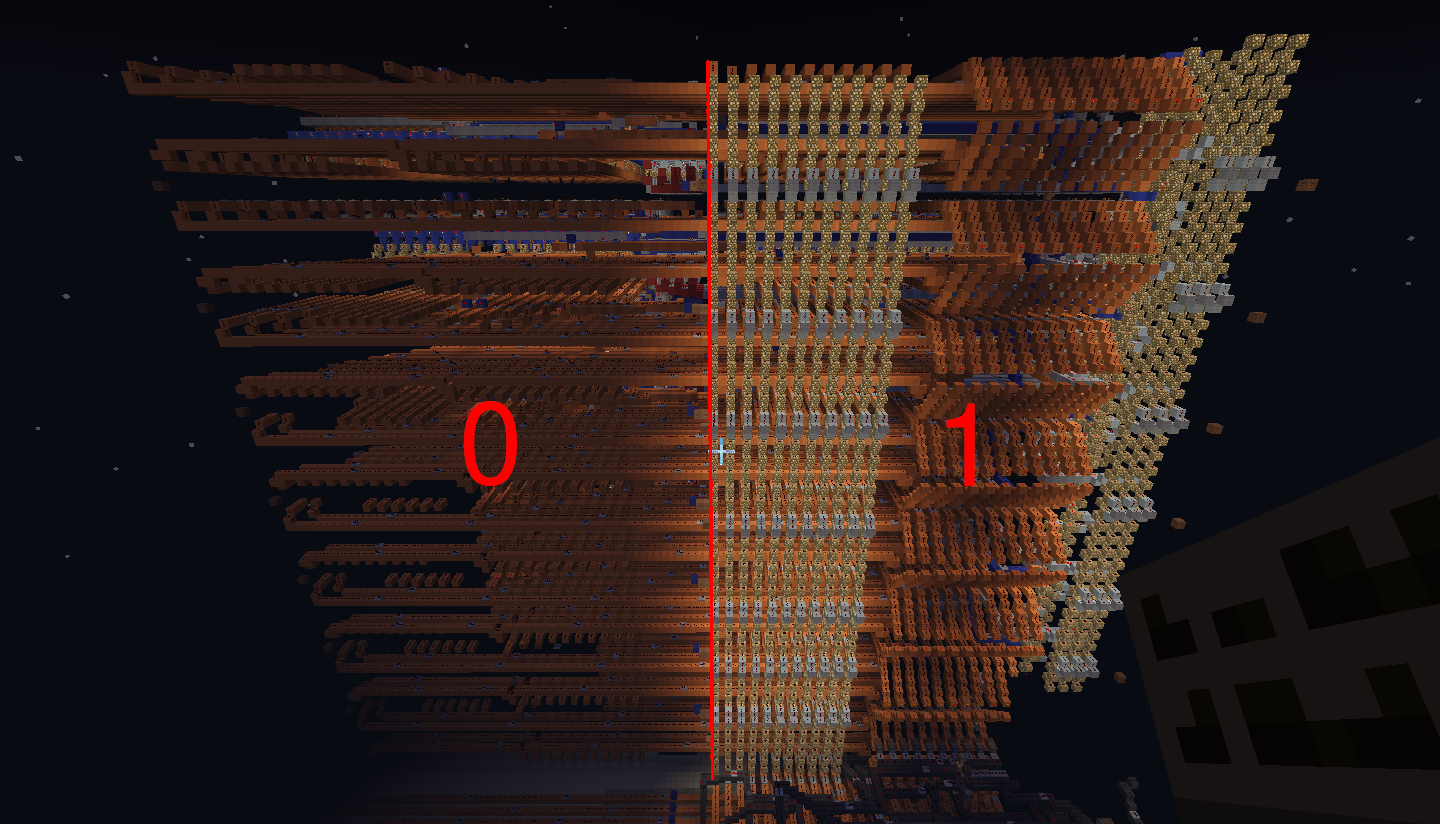
\includegraphics[width=0.9\textwidth]{Ram sides.png}
        \caption{2 sides per layer}
    \end{minipage}
\end{figure}

~\\
For selecting the right address the ram uses decoders. The ram has eight layers which all have two sides which both have sixteen addresses. The address uses the format lllsaaaa. Bit 7, 6, 5 of the address bus selects which layer the address is, bit 4 Selects in which side of the layer the address is and bit 3, 2, 1, 0 selects the address in the side in the layer. For this it uses three types of decoders. One to select the layer, one to select the side in the layer and one to select the address in the side in the layer. This is more efficient than having one big decoder, because the decoders can decode simultaneously.

~\\
The design of the RAM addresses comes from this video: \BennysRAM.
\section{ALU}
The ALU has the responsibillity to perform arrithmetic and logical operations on values.
There are four operations:
\begin{itemize}
	\item{add}
	\item{neg}
	\item{NOT}
	\item{AND}
\end{itemize}
To add the ALU uses adders. Watch this video to understand how an adder works: \adder. In binary a number can be negated by performing a NOT operation on it and then adding 1 to it. When neg is being performed it will set In1 to 0x001 which is equal to one. The NOT will be enabled wich will perform the logical operation NOT on In2. This value shall then be added with In1 wich is as previously described one. Thus the negative of In2 shall come out of the ALU. NOT works the same as Neg, except that In1 is equal to 0x000 or zero. If you understand how an adder works which you do if you have watched the video. You would know that the carry of every half adder is the same as performing the logical operation AND on the two inputs. Thus we can get an output of AND by connecting the carry bit to the ALU out. The carry lines between the half adders will be disconnected, as the different bits shouldn't have effect on each other.
\begin{figure}[h]
	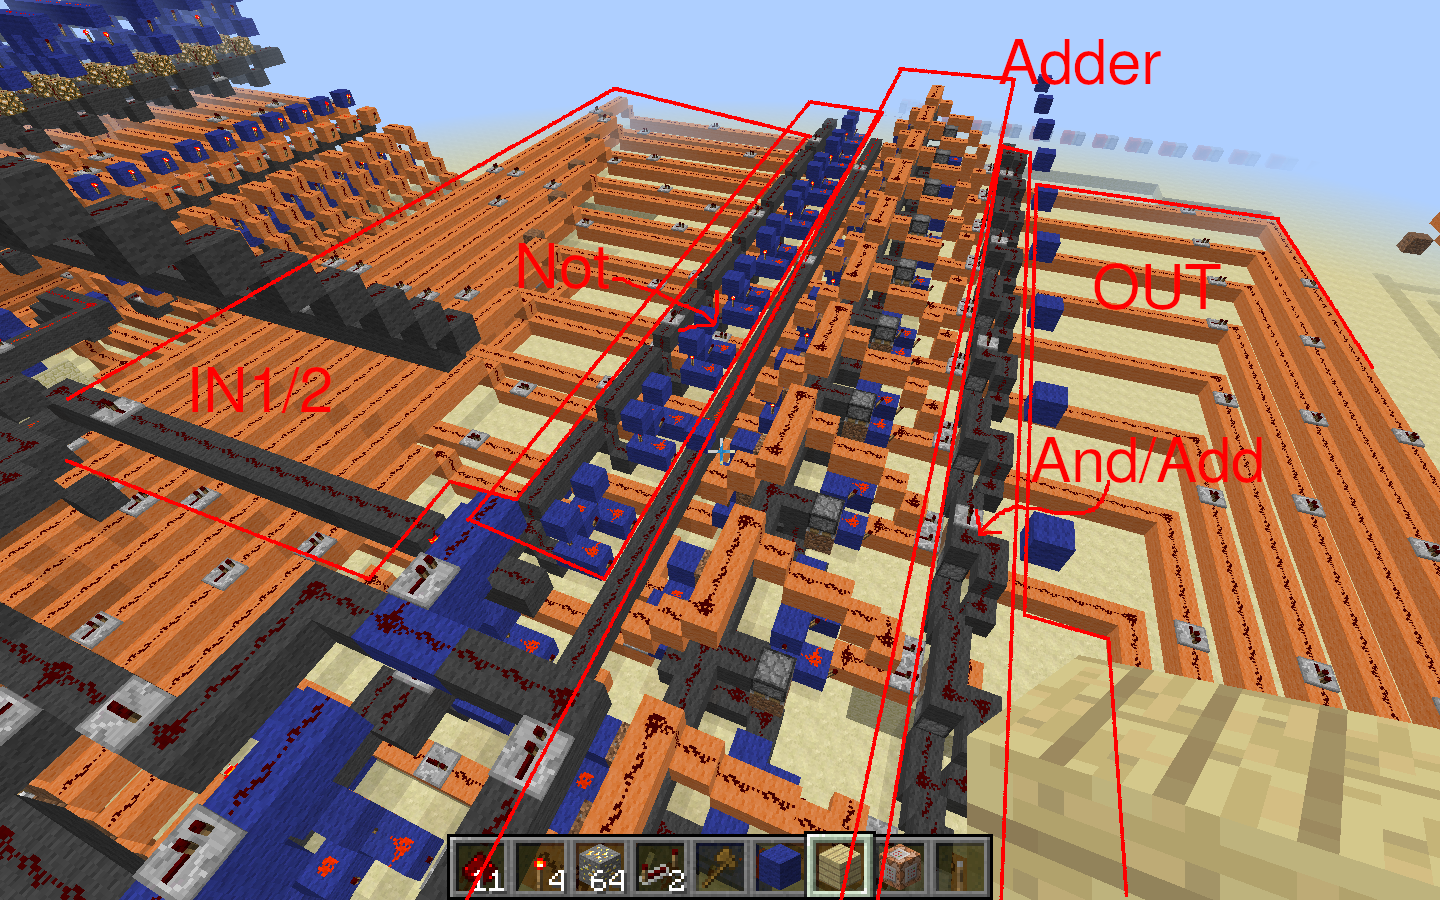
\includegraphics[width=\textwidth]{ALU3.png}	
	\caption{ALU}
\end{figure}

~\\
In this design there are many operations that are missing, but this is not a big problem as with these operations al other operations can be performed in software.
\subsection{carry\label{ALU}}
If the ALU is performing the operation add there is a possibility that the output value is to big to display with 11 bits. This is called overflow. If overflow occures the carry register shall be turned to one. If there is no overflow during addition the carry register shall be put to zero. This register is used for conditional branching (see section  \ref{SkipCarry}).
\section{Instructions}
In this section we will talk about de different instructions and how they are executed and loaded.
\subsection{Program counter}
The program counter has the task to keep track of which instruction is currently being executed or loaded. When the computer is reset, the program counter will be equal to zero. This is true for all registers.
\subsection{Instruction cycle and clock\label{Instruction cycle}}
The program that the computer runs is comprised of instructions that are executed sequentially. There are two fases in executing instructions. First is the fetch fase where it will increment the program counter by one and then load the instruction from that address and store it in to the instruction register. If it is loading the first instruction that gets executed, the program counter wont be incremented as it should load from address 0x000. 

~\\
After the fetch fase comes the execute fase which is when the instruction in the instruction register will be executed. The fetch/exec register keeps track in which fase the computer is. When it is in the execute fase it will hold the value one and if it is in the fetch fase it will hold the value zero. The clock goes on and off in a constant frequency. The clock does this to make sure that the different parts of the computer are synchronised. a Fetch/ex period is equal to two clock periods. A clock period is equal to one fase and a Fetch/ex period is equal to one loaded and executed instruction.
\begin{figure}[h]
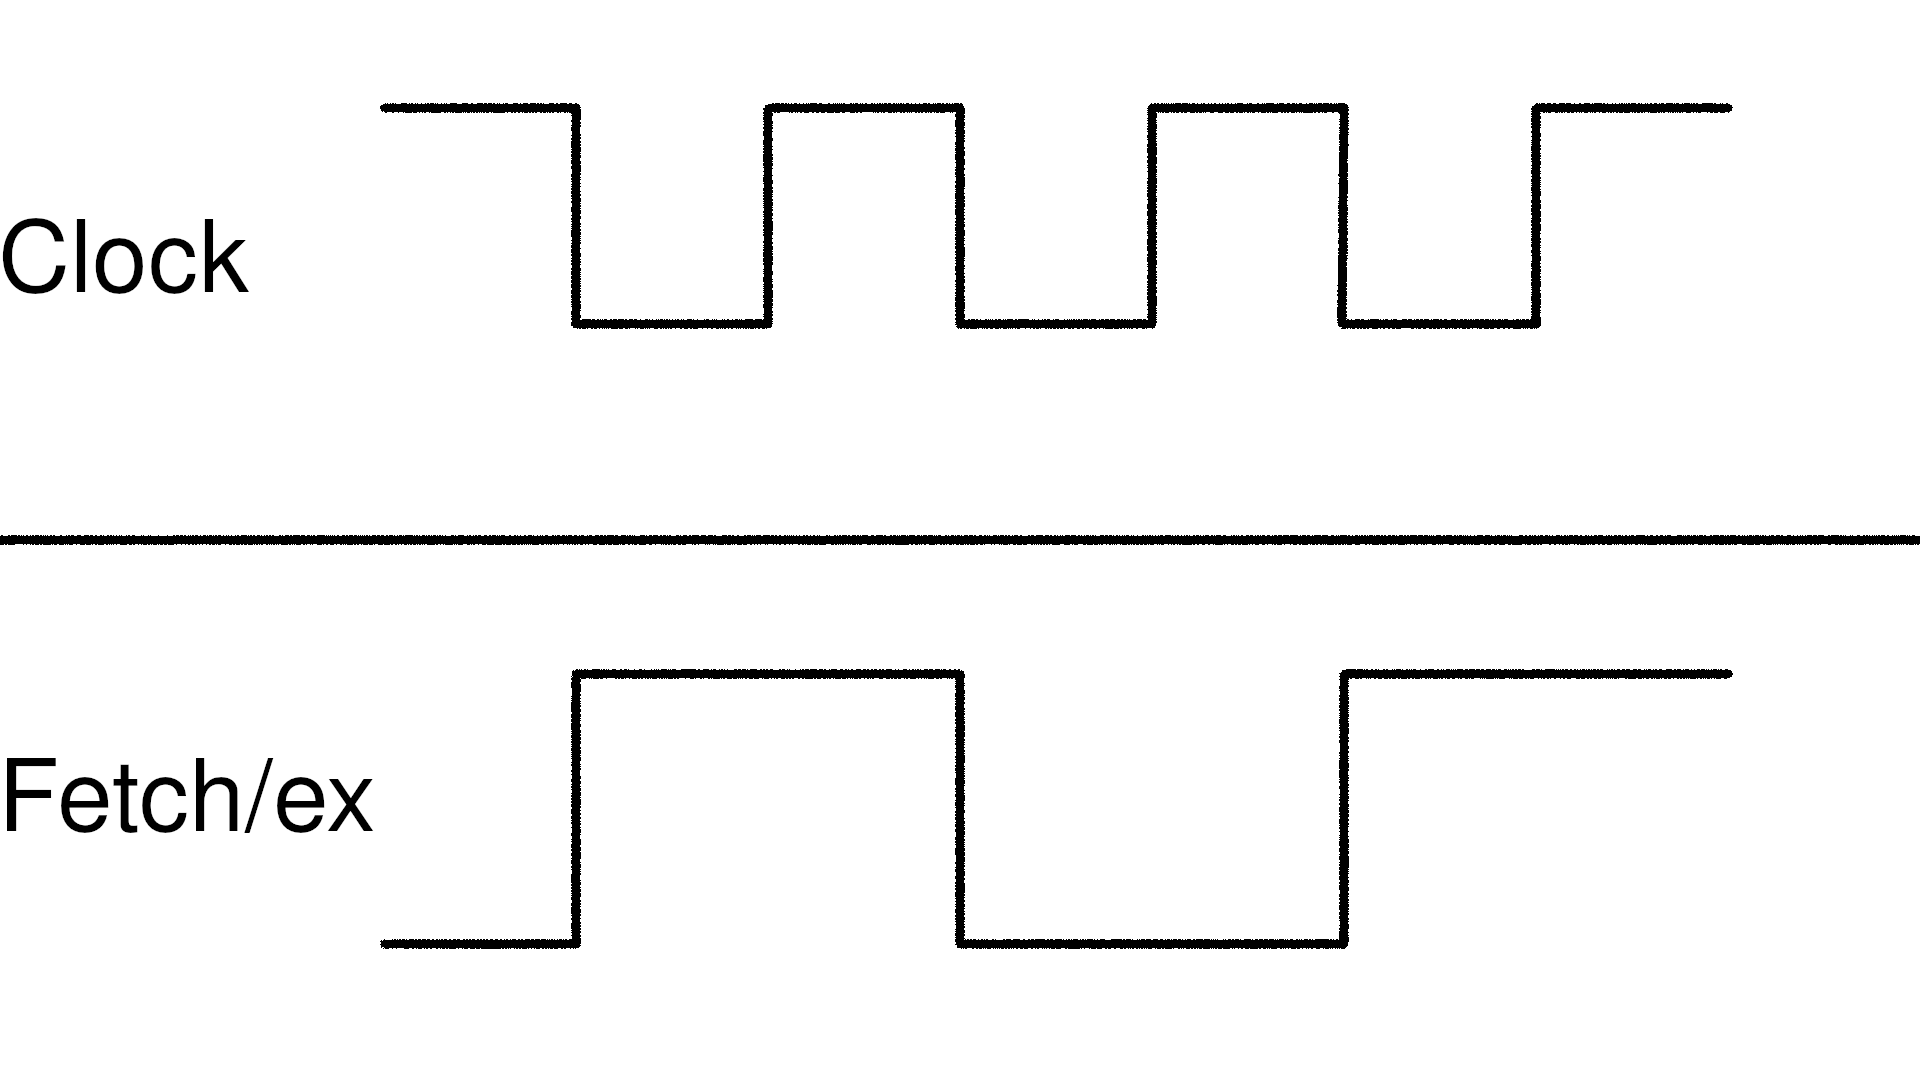
\includegraphics[width=\textwidth]{Fases.png}
\caption{shows the period of Fetch/ex compared to clock}
\end{figure}
\subsection{Accumulator}
The accumulator is a register which functons as a temporary storage location. This is necassary when there has to be an operation done with multiple values. Only one value can be loaded from RAM at a time. Thus it should load one value and store it in the accumulator and then perform the operation.
\subsection{Load}
Instruction:000 aaaa aaaa
~\\
Loads from an address in RAM and stores it in the accumulator. The a bits should be replaced with the address in RAM that it should load from.
\subsection{Store}
Instruction:001 aaaa aaaa
~\\
Loads from the accumulator and stores it in an address in RAM. The a bits should be replaced with the address in RAM it should write too.
\subsection{Add}
Instruction:100 aaaa aaaa
~\\
Loads from the accumulator and load from an address in RAM and add those values. This value is then stored back in the accumulator. Replace the a bits with the address it should load from.
\subsection{Neg}
Instruction:101 aaaa aaaa
~\\
Load from an address in RAM, negate \footnote{Making a positive number from a negative number and making a negative number from a positive number} this value and store it in the accumulator. Replace the a bits whith the address that it should load from.
\subsection{NOT}
Instruction:011 aaaa aaaa
~\\
Load from an address in RAM, perform the logical operation NOT on it and store it in the accumulator. Replace the a bits whith the address that it should load from.
\subsection{AND}
Instruction:100 aaaa aaaa
~\\
Loads from the accumulator and load from an address in RAM and perform the logical operation AND to them. This value is then stored back in the accumulator. Replace the a bits whith the address that it should load from.
\subsection{Decoding and encoding}
As said in section \ref{Instruction cycle} the current intruction is stored in the instruction register. Bit 7, 6 and 5 which specify the instruction are then send to the instruction decoder which connects with the instuction encoder. The instruction encoder describes which actions should be taken given the instrution. It is composed of of 11 lines. Eight correspond with an instruction and three correspond with a fetch operation (see section \ref{Branch}) If the fetch/ex register is turned of which is equivalent to saying that the CPU is in the fetch fase it will turn of one of the three fetch lines. If it is in the execute fase it will Every instruction has its own line that can be turned of.
\begin{figure}[h]
	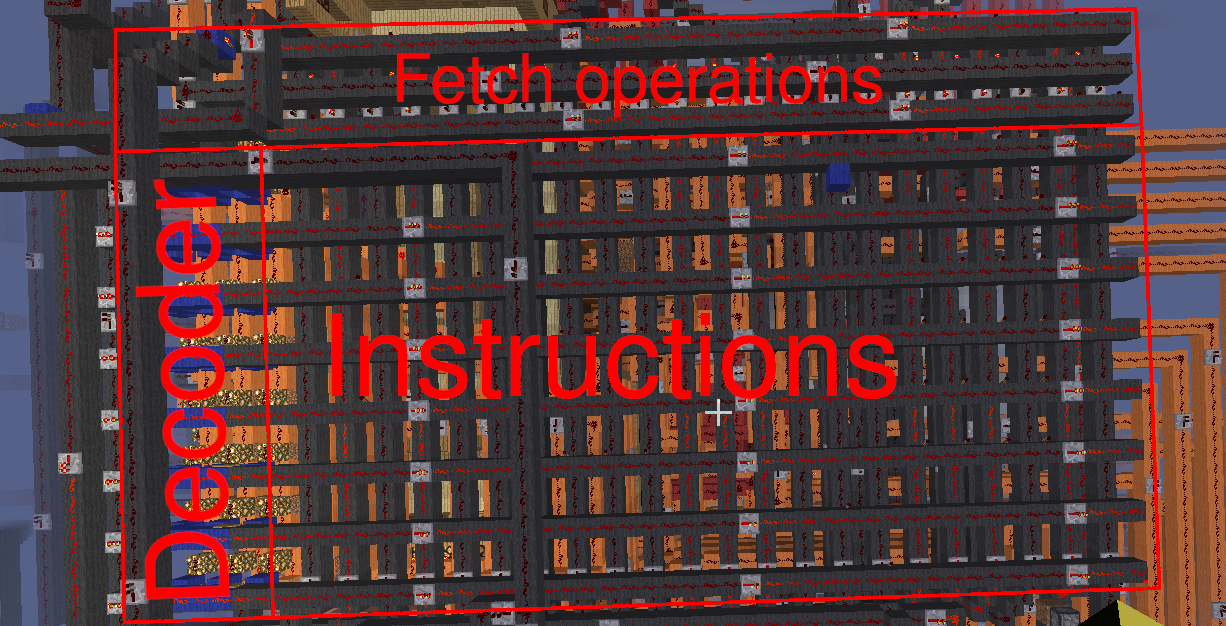
\includegraphics[width=\textwidth]{Encoder Decoder.png}
	\caption{Shows the different types of lines that the encoder has.}
\end{figure}
\subsection{Control lines}
There are in total 22 control lines which are connected between the instruction encoder and the different parts of the machine. Here is a table of all of them.
	\begin{tabular}{l l l l l l l l l l l l l }
		\hline
		name 		& num & LOAD & STORE & AND & NOT & add & neg & SKIP    \\  \hline
		ALUb=JUMP to	& 21  & 0    & 0     & 0   & 0   & 0   & 0   & 0        \\ \hline
		en IR		& 20  & 0    & 0     & 0   & 0   & 0   & 0   & 0        \\ \hline
		addr.=instr.	& 19  & 1    & 1     & 1   & 1   & 1   & 1   & 0        \\ \hline
		en RAM		& 18  & 1    & 1     & 1   & 1   & 1   & 1   & 0        \\ \hline
		ALUb=ALU	& 17  & 0    & 0     & 1   & 1   & 1   & 1   & 0        \\ \hline
		ld		& 16  & 1    & 0     & 1   & 1   & 1   & 1   & 0        \\ \hline
		jmp		& 15  & 0    & 0     & 0   & 0   & 0   & 0   & 0        \\ \hline
		skip		& 14  & 0    & 0     & 0   & 0   & 0   & 0   & 1        \\ \hline
		\hline                                                             
		Too In2.1	& 13  & 0    & 0     & 0   & 0   & 0   & 0   & 0        \\ \hline
		Too In2.0      	& 12  & 0    & 0     & 0   & 0   & 0   & 0   & 0        \\ \hline
		\hline                                                             
		addr=PC		& 11  & 0    & 0     & 0   & 0   & 0   & 0   & 0        \\ \hline
		In2=CU	        & 10  & 0    & 0     & 0   & 0   & 0   & 0   & 0        \\ \hline
		In2=RAM	        & 9   & 0    & 0     & 1   & 1   & 1   & 1   & 0        \\ \hline
		neg	        & 8   & 0    & 0     & 0   & 0   & 0   & 1   & 0        \\ \hline
		en acc	        & 7   & 1    & 0     & 1   & 1   & 1   & 1   & 0        \\ \hline
		add	        & 6   & 0    & 0     & 0   & 0   & 1   & 0   & 0        \\ \hline
		AND	        & 5   & 0    & 0     & 1   & 0   & 0   & 0   & 0        \\ \hline
		NOT	        & 4   & 0    & 0     & 0   & 1   & 0   & 0   & 0        \\ \hline
		In1=pc	        & 3   & 0    & 0     & 0   & 0   & 0   & 0   & 0        \\ \hline
		In1=acc	 	& 2   & 0    & 0     & 1   & 0   & 1   & 0   & 0        \\ \hline
		en PC	 	& 1   & 0    & 0     & 0   & 0   & 0   & 0   & 0        \\ \hline
		ALUb=RAMb	& 0   & 1    & 0     & 0   & 0   & 0   & 0   & 0            
	\end{tabular}
	continued:
\begin{center}
	\begin{tabular}{l l l l l p{6cm} }
		\hline
		name 	 	& JMP  & -norm & -jmp & -skip &Description\\ \hline
		ALUb=JUMP to    & 0    & 0     & 1    & 0     &The contents of the ``JMP to" register shall be put on the ALUb	 \\ \hline
		en IR	        & 0    & 1     & 1    & 1     &Change the value of the instruction register. \\ \hline
		addr.=ins       & 0    & 0     & 0    & 0     &Bit 7 untill 0 of the instruction goes too the address bus. \\ \hline
		en RAM	        & 0    & 1     & 1    & 1     &Enable ram \\ \hline
		ALUb=ALU        & 0    & 1     & 0    & 1     &Put the output of the ALU on the ALU bus \\ \hline
		ld	        & 0    & 1     & 1    & 1     &Read from RAM, otherwise it will write to RAM \\ \hline
		jmp	        & 1    & 0     & 0    & 0     &Enable JMP register. \\ \hline
		skip	        & 0    & 0     & 0    & 0     &Enable the skip register\\ \hline
		In2.1       	& 0    & 0     & 0    & 1     &If ``In2=CU" is also enabled it decides if bit 1 of In2 should be 1 or 0\\ \hline
		In2.0       	& 0    & 1     & 0    & 0     &If ``In2=CU" is also enabled it decides if bit 2 of In2 should be 1 or 0\\  \hline
		addr=ALUb       & 0    & 1     & 1    & 1     &Output of the ALU goes to the address bus of RAM	 \\ \hline 
		In2=CU	        & 0    & 1     & 0    & 1     &Bit 2-10 of In2 will al be 0 and 0-1 are decided by In2.1 and In2.0\\ \hline
		In2=RAM	        & 0    & 0     & 0    & 0     &The output of ram will be put in In2.	 \\ \hline
		neg	        & 0    & 0     & 0    & 0     &Output of ALU is negative of In2	 \\ \hline
		en acc	        & 0    & 0     & 0    & 0     &Change the value of accumulator	 \\ \hline
		add	        & 0    & 1     & 0    & 1     &Output of ALU is sum of In2, In1	 \\ \hline
		AND	        & 0    & 0     & 0    & 0     &Output of ALU is AND on In2, In1	 \\ \hline
		NOT	        & 0    & 0     & 0    & 0     &Output of ALU is NOT on In2	 \\ \hline
		In1=pc	        & 0    & 1     & 0    & 1     &In1 is the contents of PC	 \\ \hline
		In1=acc	        & 0    & 0     & 0    & 0     &In1 is the contents of accumulator	 \\ \hline
		en PC	        & 0    & 1     & 1    & 1     &Change the value of PC	 \\ \hline
		ALUb=RAM	& 0    & 0     & 0    & 0     &Puts output of RAM on ALU bus	 \\ \hline
		\hline
	\end{tabular}
\end{center}

\section{Branching\label{Branch}}
\subsection{JMP}
Instruction:111iiiiiiii
~\\
When the JMP instruction is executed the JMP register shall be turned to one and bits i bit of the instruction (bit 0-7) shall be stored in the ``JMP to" register. Because the JMP register is set to one, the instruction -jmp shall be executed instead of -norm during the next fetch fase. What this means is that it won't go to the next instruction as would normally happen, but to the instruction specified by the jmp instruction.
\subsection{Skip\label{SkipCarry}}
Instruction:110bbbbzcsx
~\\
When the Skip instruction is executed the Skip register shall be turned to one if a certain condition is met. If the skip register is turned on the PC register shall be incremented by two instead of one in the next fetch fase, thus skipping an instruction. There are three posible conditions:
\begin{itemize}
	\item{Zero}
	\item{Carry}
	\item{Bit}
\end{itemize}
If you want the zero condition you should turn on bit z (bit 3). If this condition is selected the skip register shall be turned to one when the value stored in the accumulator is zero.

~\\
If you want the carry condition you schould turn on bit c (bit 2). If this condition is selected the skip register shall be turned to one if the carry register is on (see \ref{ALU}).

~\\
If you want the Bit condition you should turn on bit s (bit 1). This will check a specified bit in the accumulator. You specify the bit of the accumulator you want to check with the b bits (bit 4-7). If the specified bit is one it will turn the skip register on.

~\\
If the skip register is on the -skip instruction shall be performed in the next fetch fase, otherwise it will perform the -norm instruction as usual.
\section{Control Room\label{UI}}
The Control Room has two spaces: The debugging room and the read/writing room.
\begin{figure}[h]
    \centering
    \begin{subfigure}{0.5\textwidth}
        \centering
        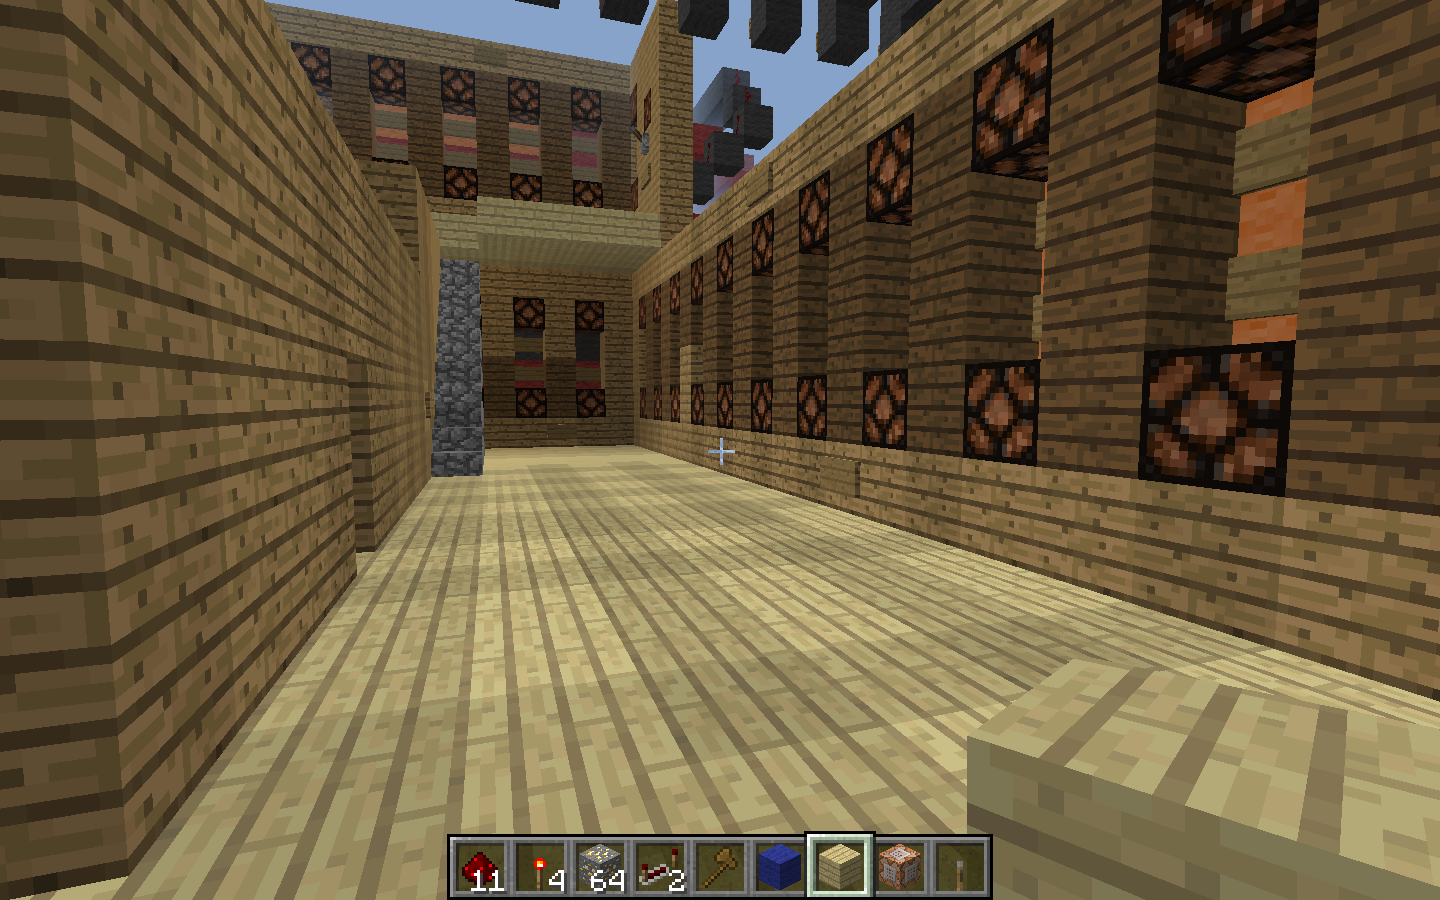
\includegraphics[width=0.9\textwidth]{Debug.png} % first figure itself
        \caption{Debugging room}
    \end{subfigure}\hfill
    \begin{subfigure}{0.5\textwidth}
        \centering
        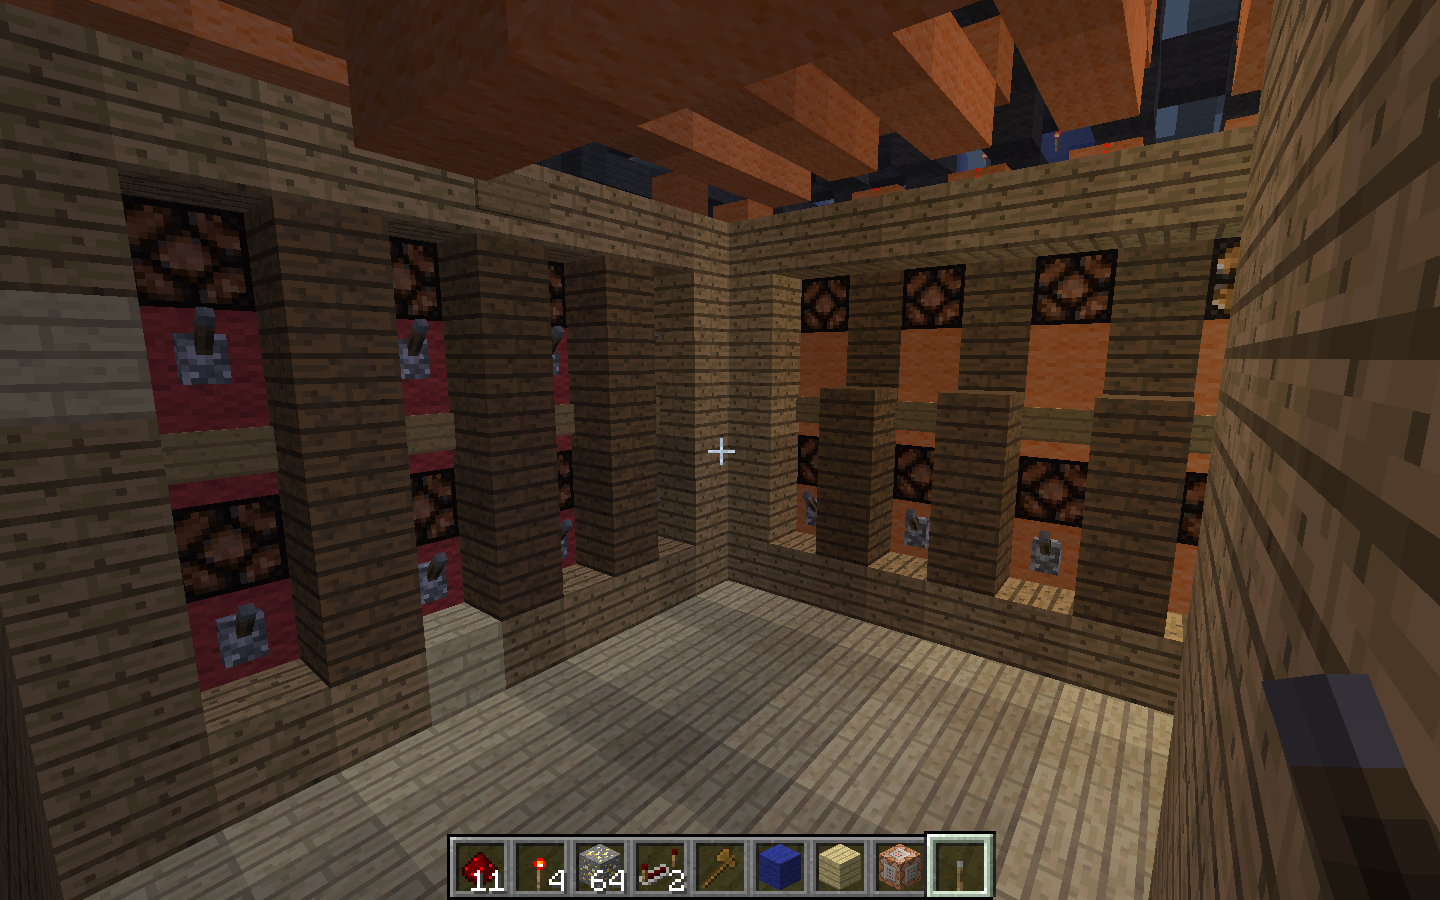
\includegraphics[width=0.9\textwidth]{ReadWrite.png} % second figure itself
        \caption{Read/Writing room}
    \end{subfigure}
\end{figure}
~\\
As the name suggests the debugging room is the place where one would debug the machine. There are indicator lights which display the contents of the different registers. In figure \ref{PC}, \ref{Flag} and \ref{Uclock} you can see which registers are displayed.
\begin{figure}[h]
	\centering
	\begin{subfigure}{0.5\textwidth}
		\centering
		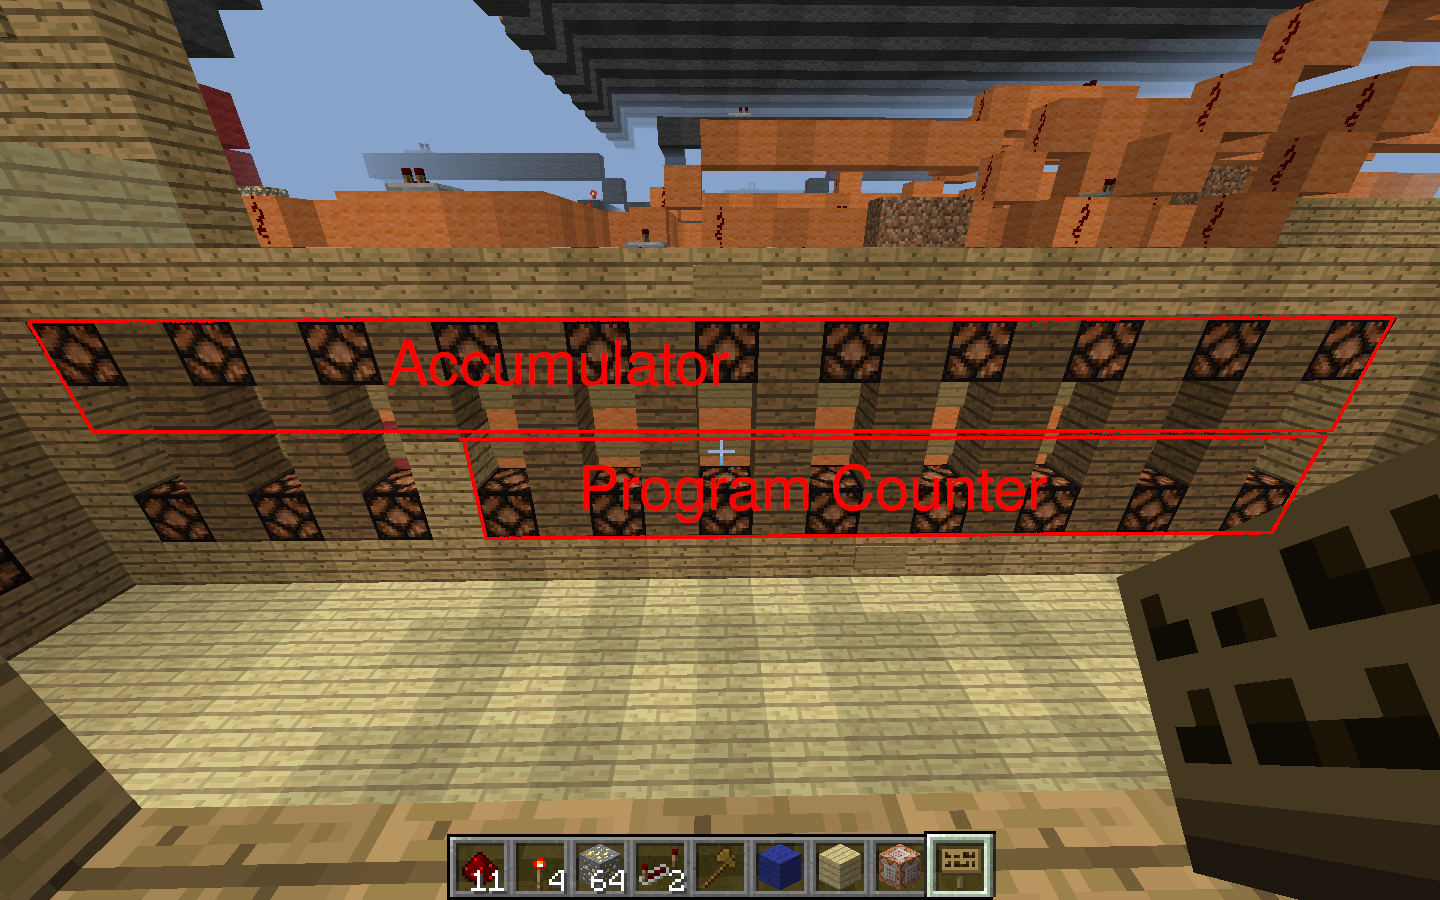
\includegraphics[width=\textwidth]{UI Acc and PC.png}
		\caption{The PC register and accumulator\label{PC}}
	\end{subfigure}\hfill
	\begin{subfigure}{0.5\textwidth}
		\centering
		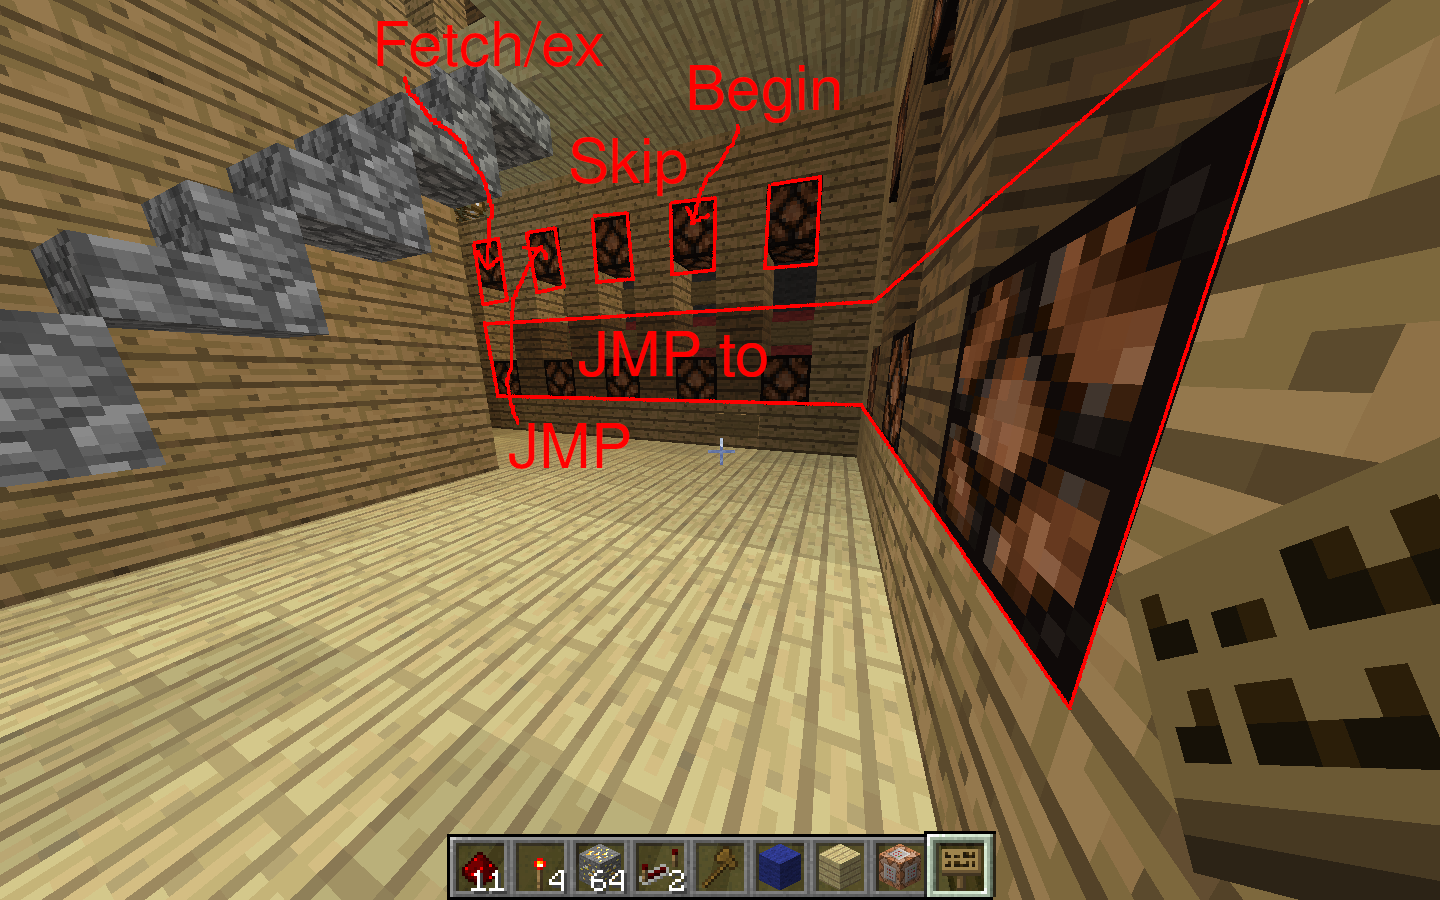
\includegraphics[width=\textwidth]{Flags.png}
		\caption{The flag registers\label{Flag}}
	\end{subfigure}
\end{figure}
~\\
If you want to debug the machine it would be nice if you could pause the computer. The leaver in figure \ref{Uclock} can be used to switch the computer between running and paused. When the system is paused you can use the button on the left to change the clock from an on to an off state or vice versa.
\begin{figure}[H]
	\centering
	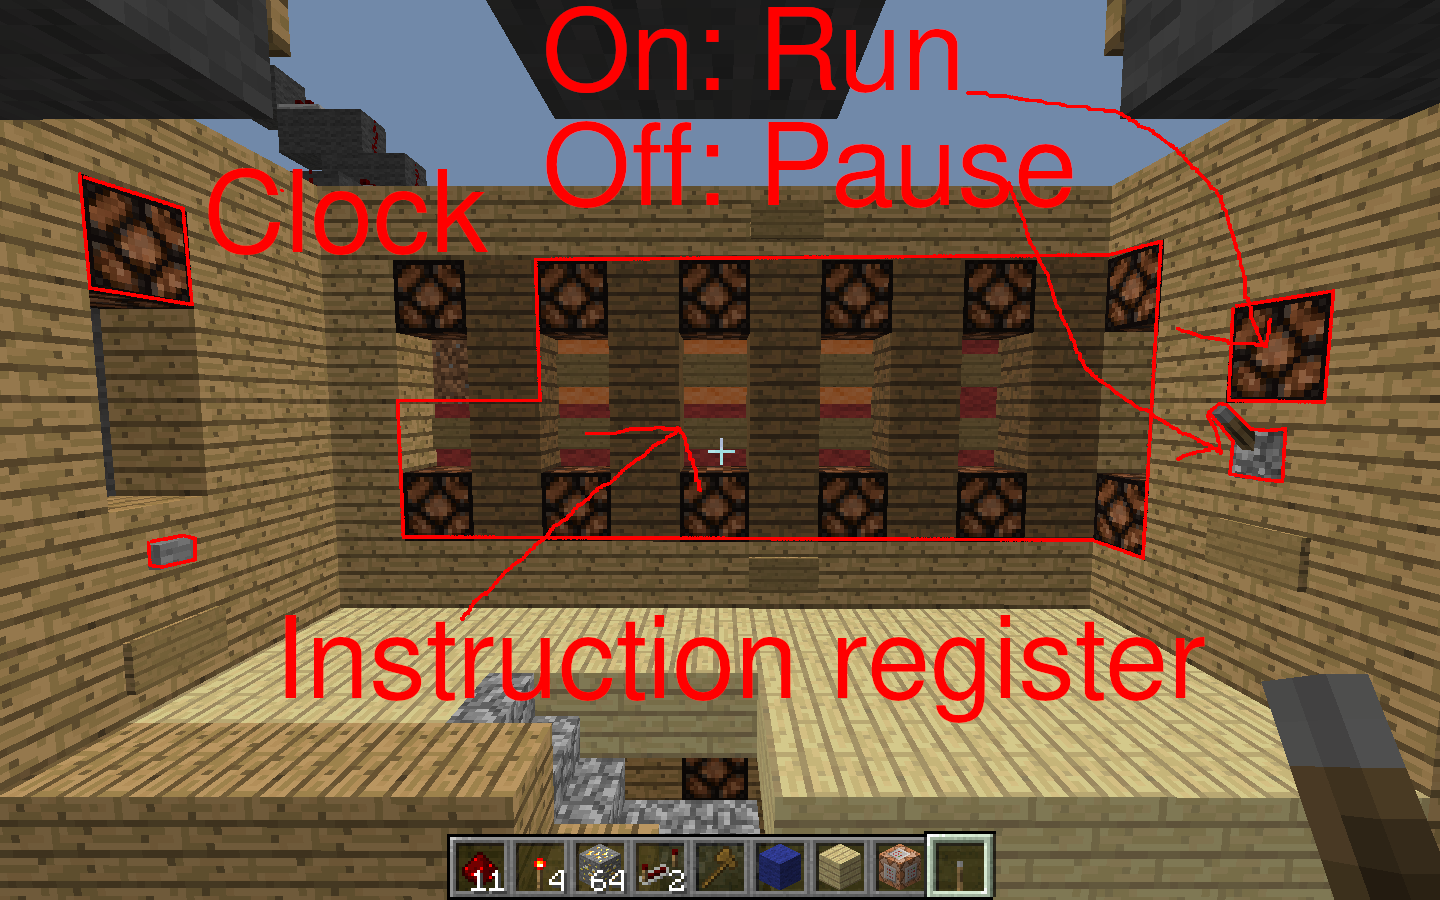
\includegraphics[width=\textwidth]{UI clock.png}
	\caption{Instruction register and clock\label{Uclock}}
\end{figure}
~\\
In figure \ref{door} you see two switches. The reset switch and the programming/run switch. The reset switch sets all registers to zero. It will in other words restart the machine. It will not reset the RAM though. The other switch is usefull when you would like to edit the contents of RAM. This will disconnect the RAM from the CPU it will also open the door to the write door.

~\\
In the write room you can read or edit the contents of RAM. Before you go into the write room make sure you have paused the machine and switched the programming/run switch to programming. This will open the door to the write room. As previously mentioned you can edit the contents of RAM in this room. To do this you should specify the RAM address you want to edit: figure \ref{Uaddress}. You can see what is currently in that address in the RAM out and can store something at that address with the switches of the RAM in. Additionally you have to switch the enable write switch and you should see see the value you've put in the RAM come in the RAM out after a while. When this is the case you know that you have succesfully written to RAM. Make sure to put switches to an off state when you leave the room, otherwise the signal would interfere with that of the CPU which will cause unpredictable behaviour.

\begin{figure}[h]
	\centering
	\begin{subfigure}{0.35\textwidth}
		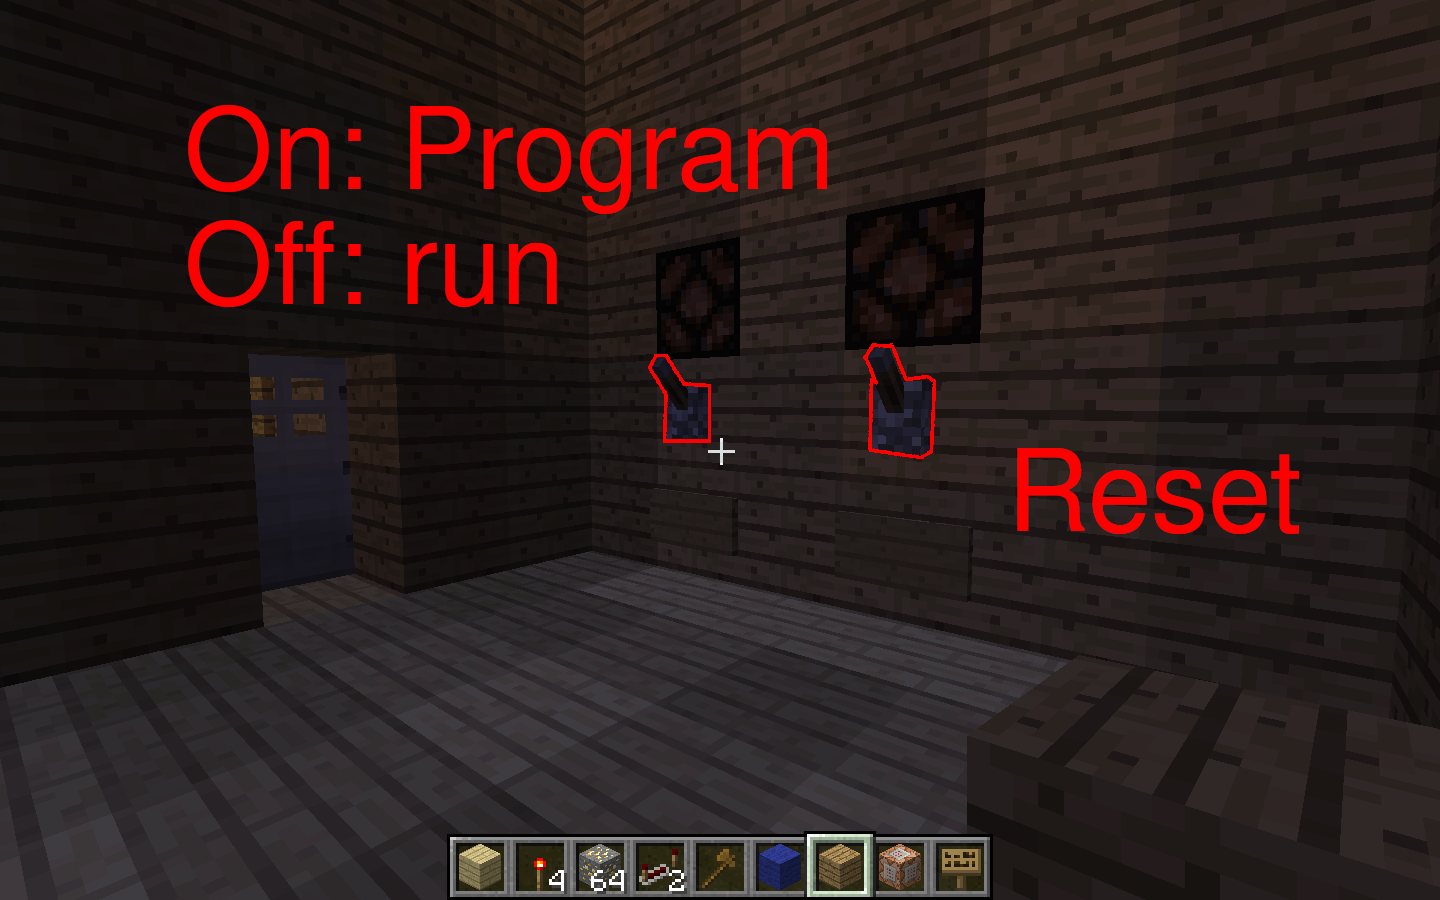
\includegraphics[width=\textwidth]{WriteDoor.png}
		\caption{Door to the write room.\label{door}}
	\end{subfigure}\hfill
	\begin{subfigure}{0.3\textwidth}
		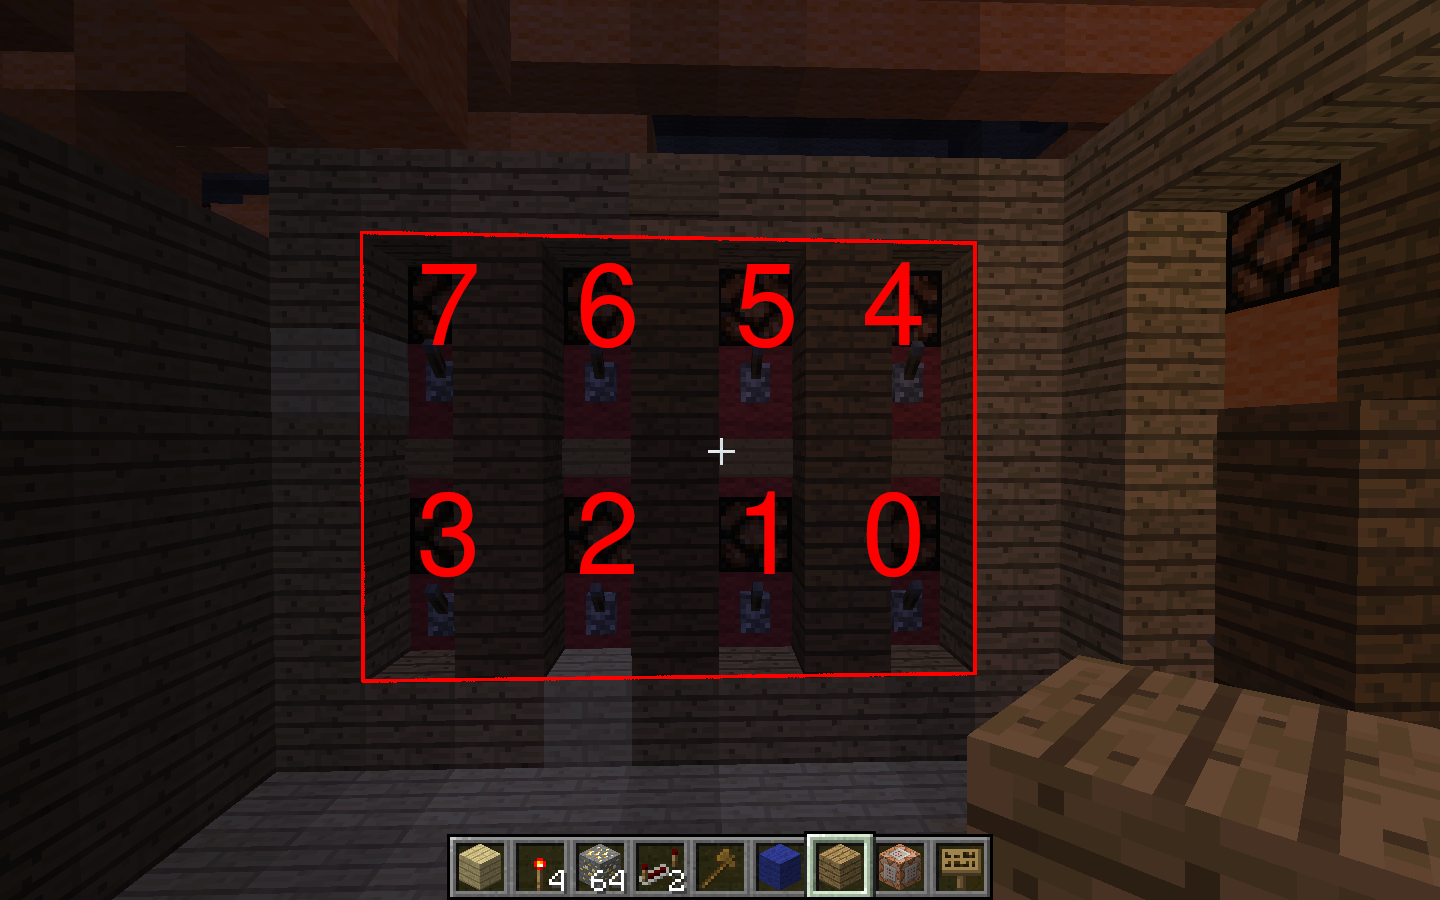
\includegraphics[width=\textwidth]{UIaddress.png}
		\caption{Here you specify the address.\label{Uaddress}}
	\end{subfigure}
	\begin{subfigure}{0.3\textwidth}
		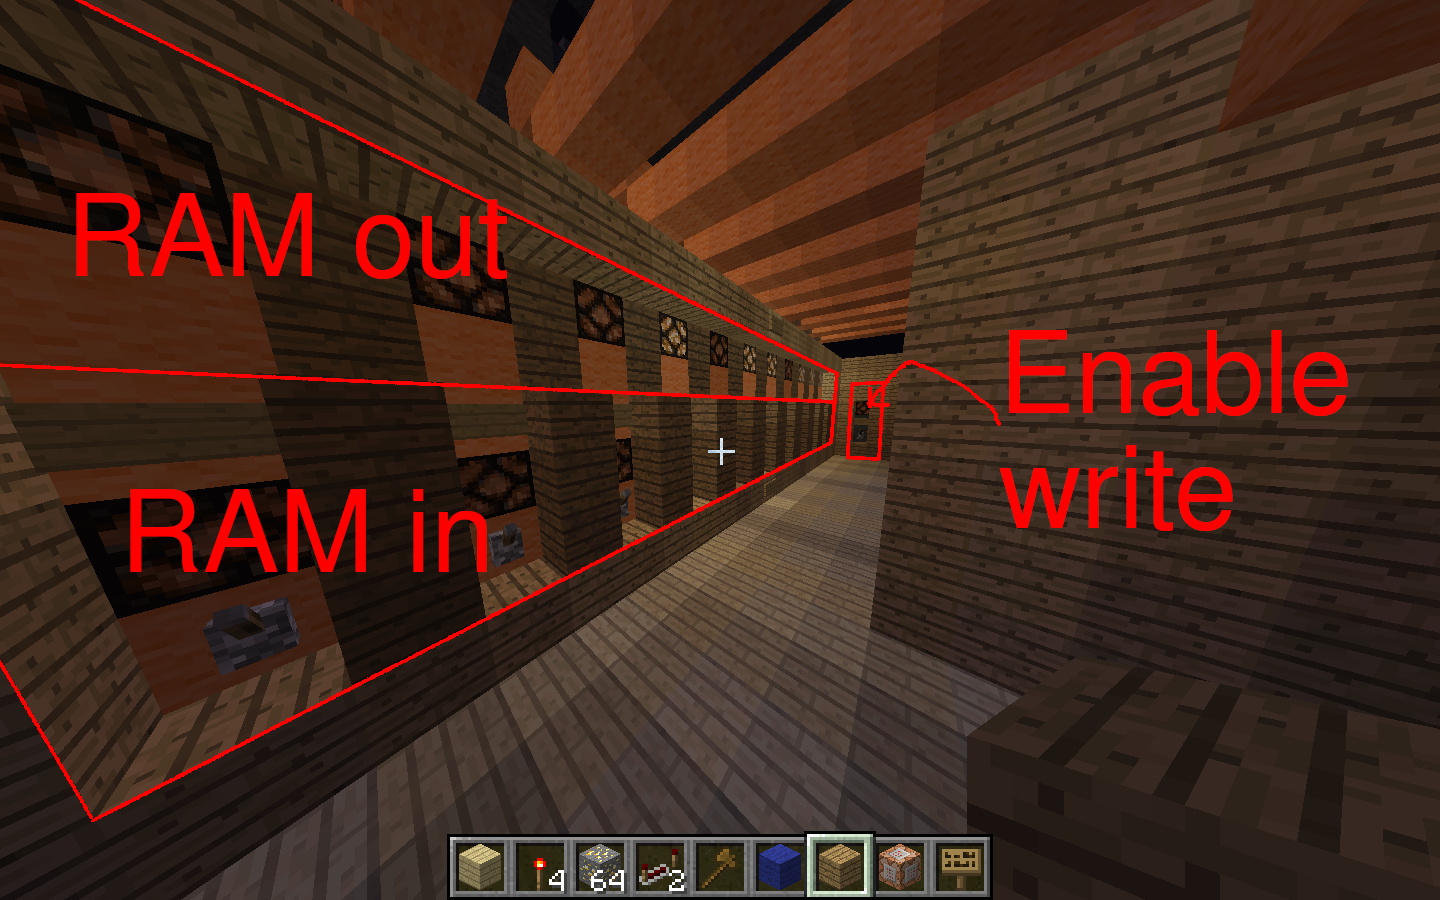
\includegraphics[width=\textwidth]{UI Ram io.png}
		\caption{Here you write to RAM.}
	\end{subfigure}
	
\end{figure}

%\begin{tabular}
%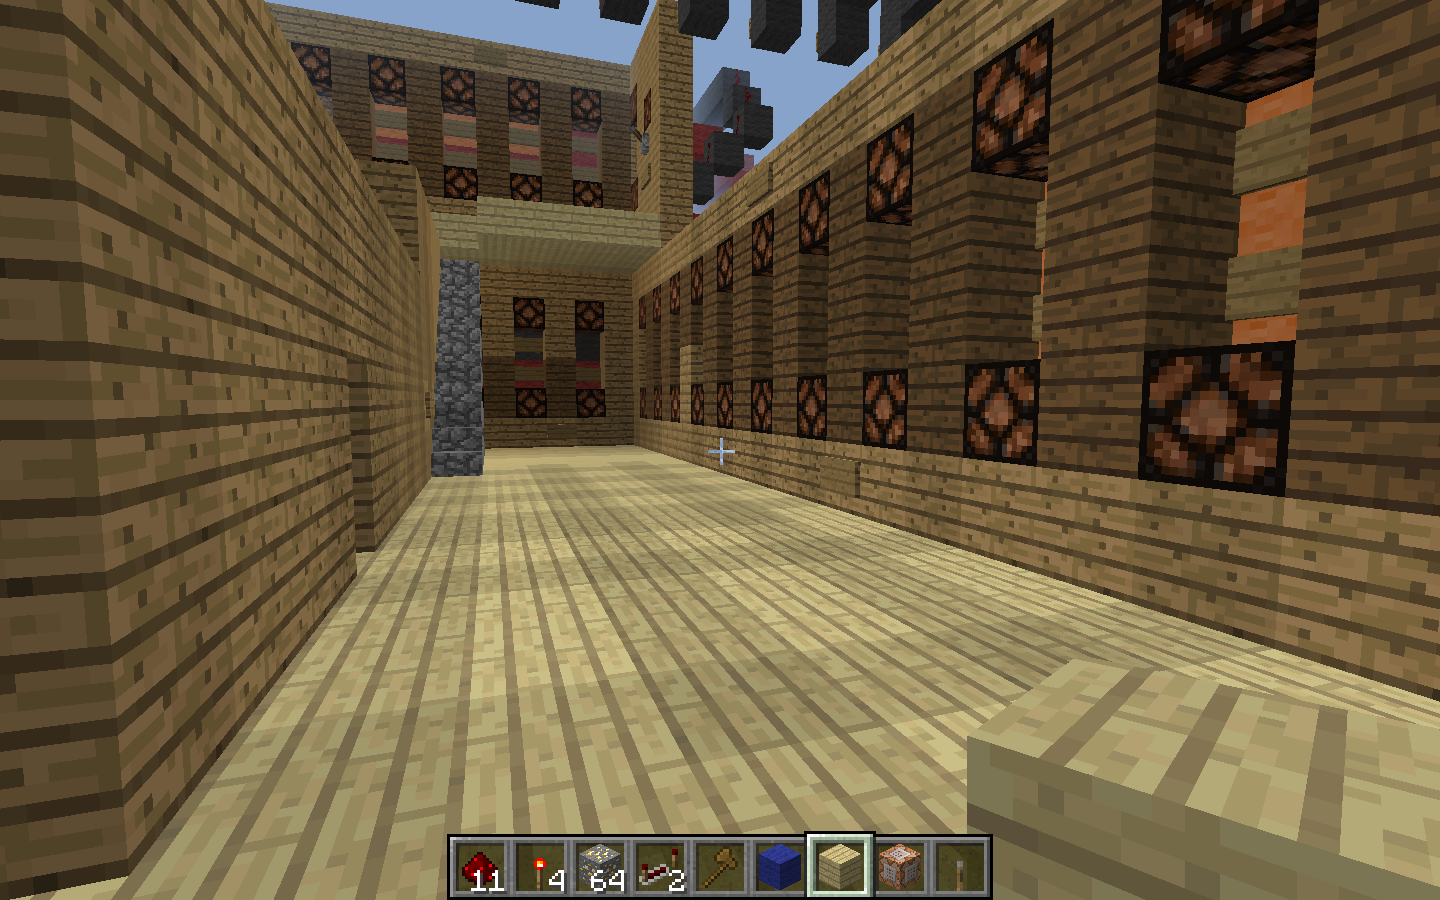
\includegraphics[width=0.5\textwidth]{Debug.png}
% &
%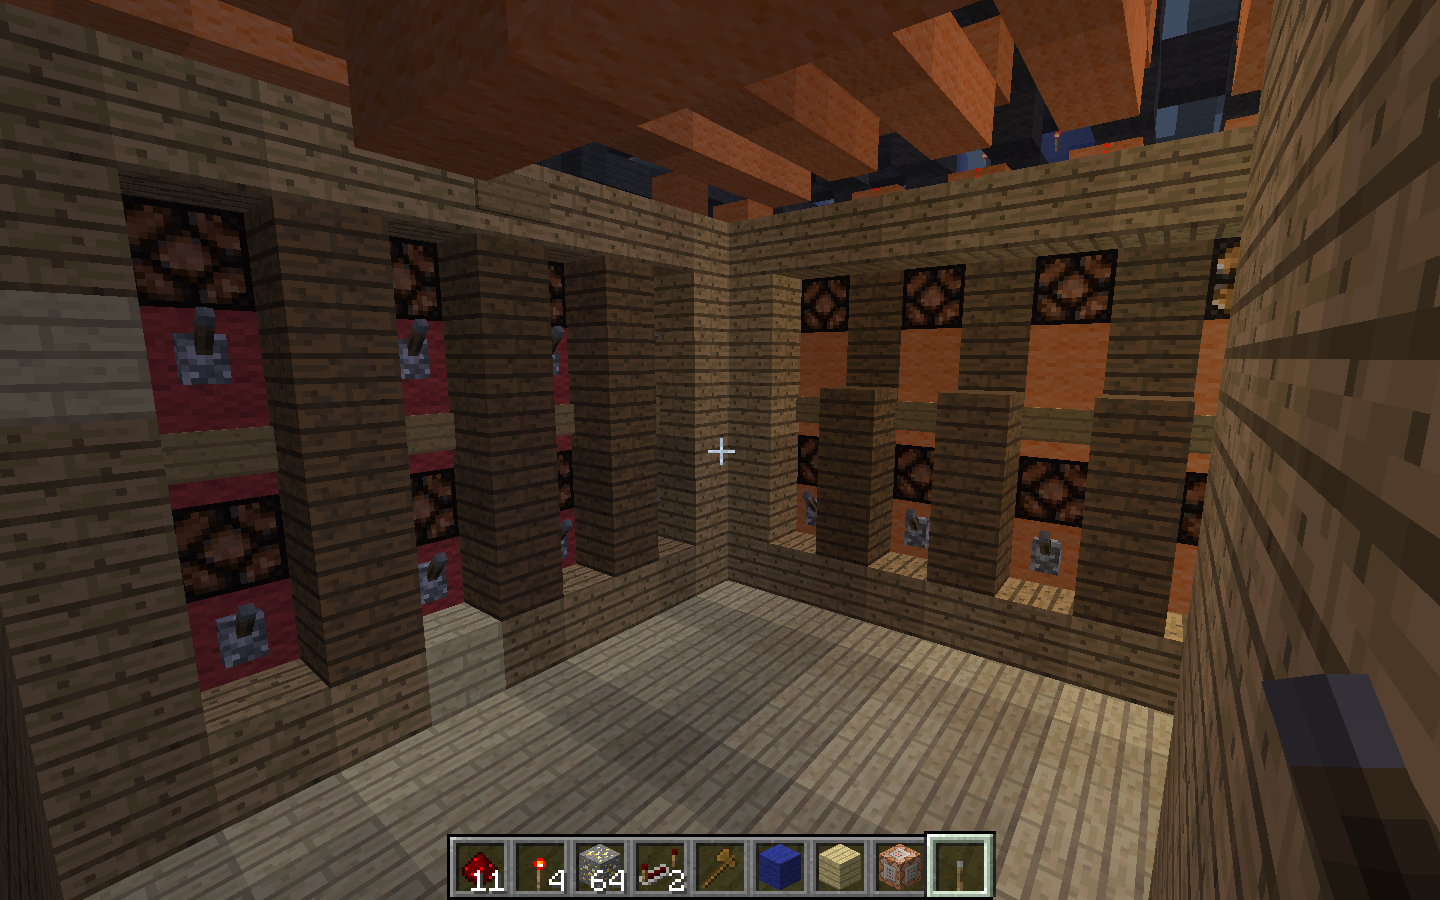
\includegraphics[width=0.5\textwidth]{ReadWrite.png}
%\end{tabular}

\section{Writing software}
\subsection{Writing techniques}
The most straitforward way of writing software for this machine might seem to just put in the program with the switches in the read/writing room and then debugging it and edit it as you go. This is inefficient, as it is easy to loose the big picture as it can be hard to read the code in binary. Debugging the program on the minecraft computer is a verry slow process including the fact that when you forgot to write one instruction say in address 123 you must move up all the instructions that come after it which all takes a long time. In this section we will discuss how we can program the machine more efficiently.
\subsection{Assembler\label{assembler}}
An assembler converts assembly language into machine code (binary instructions). Assembly language is a way of making machine code more human-readable. Instead of binary it uses names for the different instructions. It also uses variables to make it easier to read the specified addresses. This is usefull, because if you change the position of a certain variable or instruction. You don't have to look through all the instructions and change everything manually, but you can just change the position of the variable and your finished.

~\\
For this purpose I wrote an assembler which you can download from my website at \assembler. If you use Mac os, linux or any other unix based operating you should go to the directory of the assembler in your terminal and execute the commnand: ``python assembler.py''. On windows it could be a bit more complicated. Read this article to learn how to run a python file on windows: \PyHow. If you use any other operating system you are probably smart enough to figure it out yourselve.

~\\
Before you can assemble your first program you first have to write the assembly code. You can write this in any text editor like vim, emacs or notepad++. The first thing you need to understand is that you have different sections in the code. One is named ``var" and another is called ``pgm". You start a section by making a line with the word ``pgm" or ``var" on it. Every line under the section specifier ``pgm" or ``var" whill be part of that type of section. Untill another specifier is found.

~\\
Commments are usefull to explain your code, so you or someone else can understand how your code works. You make a comment by placing a '/' a comment by writing a ‘/’. All text that is on the same line and comes after the ‘/’ shall then be ignored.
\begin{figure}[H]
	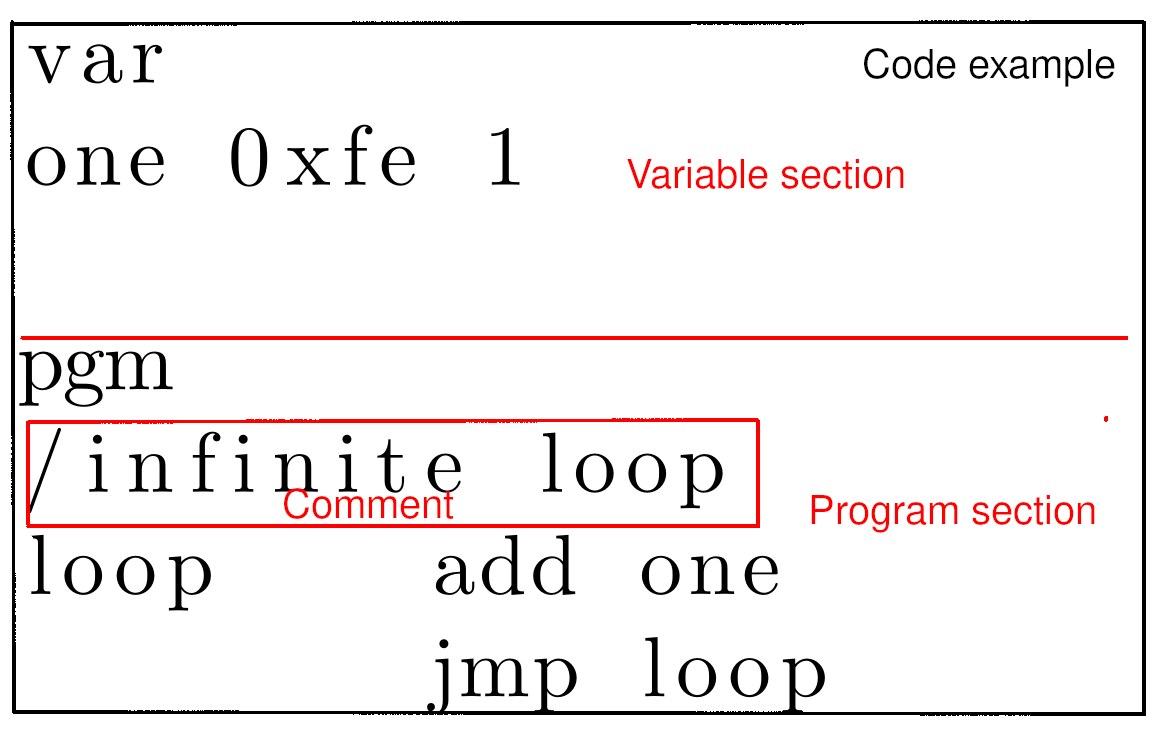
\includegraphics[width=0.5\textwidth]{Comments and sections.png}
\end{figure}
~\\
In the pgm section the user makes a list of instructions. The uppermost instruction shall be mapped with address zero and the second uppermost shall be mapped with address one and so on. If you have to many instructions the assembler shall give an error message as there are only 256 addresses in the RAM of the computer. You can only write one instruction per line, but you are allowed to keep lines empty. In most cases you must start your instruction with the name of the instruction. The possible instruction names are:
\begin{itemize}
	\item{load}
	\item{store}
	\item{add}
	\item{neg}
	\item{NOT}
	\item{AND}
	\item{jmp}
	\item{skip}
\end{itemize}
These obviously correspond with the 8 instructions that the computer has. For the instruction load, store, add, neg, NOT and AND You have to specify an address. There are several ways of specifying an address. You can give the name of variable specified in the ``var" section or an instruction label specified in the ``pgm" section. It is important that the variable is defined before the instruction, but the instruction label doesn't need to be defined before the instruction. The other option is to specify the address. You would mostly specify the address in decimal. You can also specify it in hexadecimal by starting the value with  ``0x" or in binary by starting with ``0b".
\begin{lstlisting}
/code example
var
variable 255 12

pgm
begin	load variable/a variable
	add 255/a decimal number
	store 0xff/a hexadecimal number
	neg 0b11111111/a binary number
	jmp begin/an instruction label
\end{lstlisting}
~\\
The instruction jmp also requires an address to be specified, but this would mostly be an instruction instead of a variable. To do this efficiently you can use instruction labels. These are similar to variables as they specify an instruction, but different because they are linked to an instruction instead of a variable. To make an instruction label you can start an instruction with the name of the label instead of an instruction. It is required that the label doesn't have the name of any of the instructions.

~\\
The instruction skip is a more special instruction. You specify the letter that corresponds to the condition. Here is the list of all conditions with the corresponding letter.
\begin{itemize}
	\item{s	bitselect}
	\item{z	zero}
	\item{c	carry}
\end{itemize}
If you choose ``s" or ``bitselect" you must also choose which bit you want as condition. You have to do this in decimal by giving a value between 0 and 7.
\begin{lstlisting}
/code example
pgm

begin	skip z/skip if accumulator is equal to zero
	skip s 4/skip if bit 4 is 1
	skip c/skip if carry register is 1
	skip s 9/skip if bit 9 is 1
	jmp begin/jmp to instruction 0
\end{lstlisting}
~\\
In the var section you give a list of variables. You can only create one variable per line. You start by giving the name of the variable. After this you give the position of the variable in RAM. You can specify this in binary, hexadecimal or decimal. Finally you should specify which value should be stored in that variable when the program is assembled which is called ``the starting value".
\begin{lstlisting}
/code example
var
/name		/position	starting value
Chickens	0xff		23
Hens		0xfe		0xa
Humans		253		0b11
\end{lstlisting}
When you run the assembler it will ask you to specify the file you want to assemble. It then asks you to specify the name of the file it will output to. It will assemble the specified file whereafter it will either give an error message which means you have to fix something or it will just stop running which means it has succesfully assembled. If it has succesfully assembled two new files should appear in the current directory. One with the specified output filename and one with the specified output filename and `` logisim" appended to it. The first file is a list of the instructions in the program and the second one can be run in logisim (see section \ref{logisim}).


\subsection{Logisim\label{logisim}}
Debugging the machine in minecraft is very time consuming. That is why I made a clone of this machine in logisim. Logisim is a digital logic simulator and the computer is a lot faster in logisim than in minecraft. I therefore advice you to debug your code in logisim. First you install logisim and then download the computer file here: \LogComp. You open that file in logisim and you should see something like in figure \ref{logisimI}.

\begin{figure}[h]
	\centering
	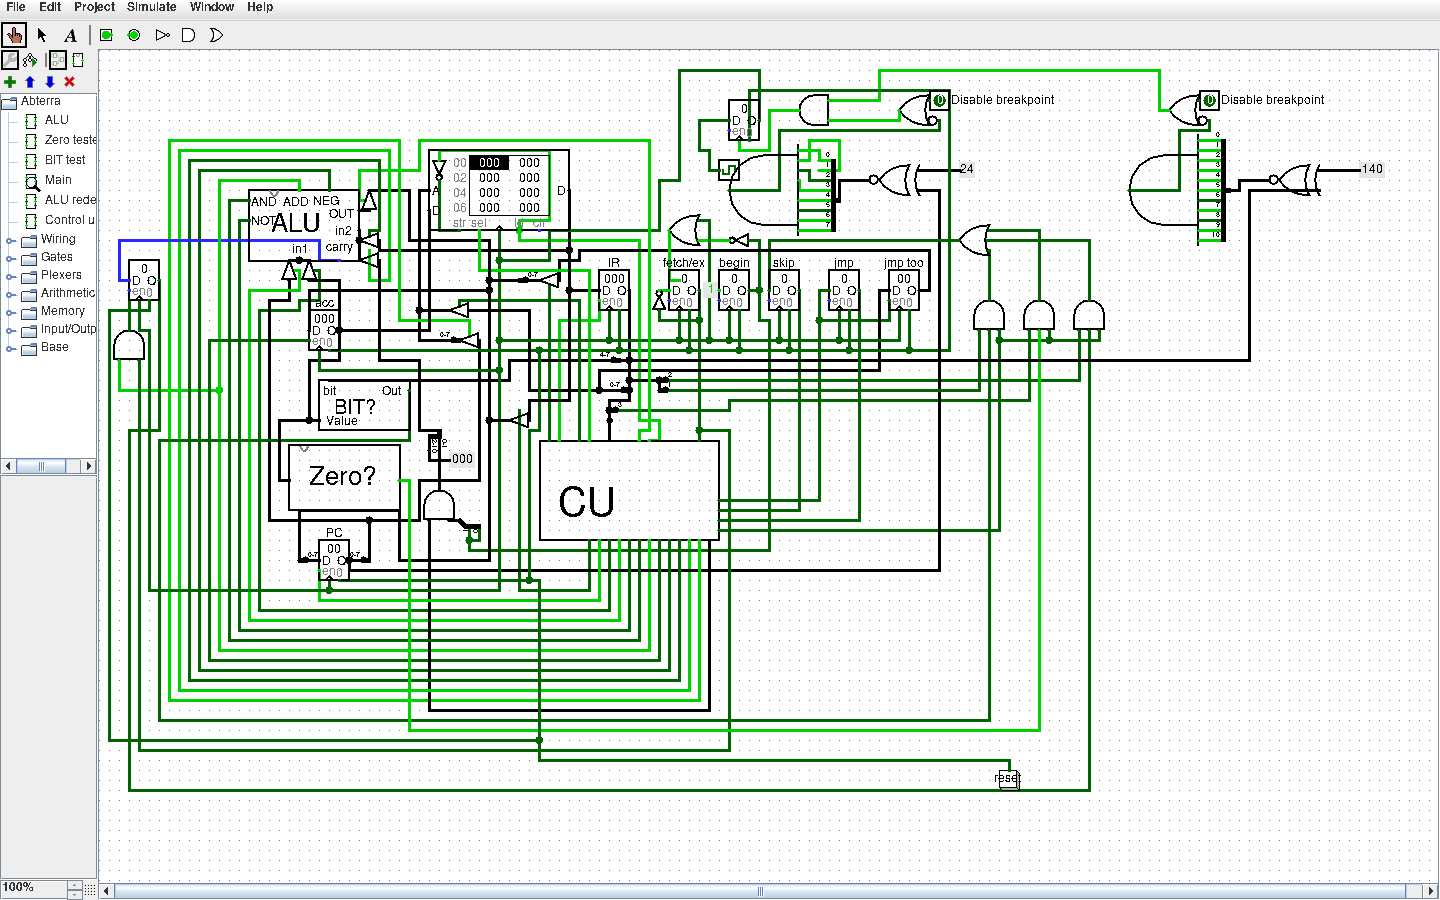
\includegraphics[width=\textwidth]{Logisim.png}
	\caption{Abterra I in logisim\label{logisimI}}
\end{figure}
~\\
To load in the program you should right-click on the RAM wherafter a menu will pop up where you should to select ``Load Image". You should then select the assembled file with `` logisim" appended to it. To then run this program first make sure to click on the ``reset" button at the bottemleft of your screen to make sure all the registers are set to zero. Then click on ``simulate" on the top left of your screen wherafter you should click on ``Ticks Enabled". This will make the clock start ticking. You can change the frequency of the ticking in ``Tick Frequency". If you have ticks disabled you can manually tick the clock by pressing ``Tick Once" By reading the values in the registers and enabling and disabling the clock you are able to debug the machine. If you have ever debugged a program before, you might have heard of the term breakpoint. a breakpoint is a place in code you define where the computer should stop executing. This is interesting when you want to debug a specific section section of the code, but you don't want to stop the computer manually at a certain point. To make a breakpoint turn of the disable breakpoint pin by pressing on it. There are two two breakpoint sections in this computer. One is called ``PC break" and will stop the clock when the machine is at a certain instruction. The other one can be connected to any register in the coputer, but it requires knowledge about logisim to use it properly so we won't discuss it here. To set the address of the breakpoint press ctrl-2 to go into edit mode and click on the constant seen in figure \ref{Break} and change its value in the selection menu. If the pc register has that value the clock will be disconnected from the computer, to connnect it again disable the breakpoint or change the break address.
\begin{figure}[h]
	\centering
	\begin{subfigure}{0.2\textwidth}
		\centering
		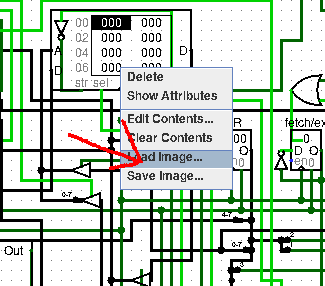
\includegraphics[width=\textwidth]{load image.png}
		\caption{The PC register and accumulator\label{PC}}
	\end{subfigure}\hfill
	\begin{subfigure}{0.1\textwidth}
		\centering
		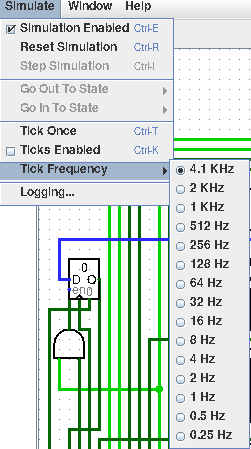
\includegraphics[width=\textwidth]{tick settings.png}
		\caption{Tick settings}
	\end{subfigure}
	\begin{subfigure}{0.6\textwidth}
		\centering
		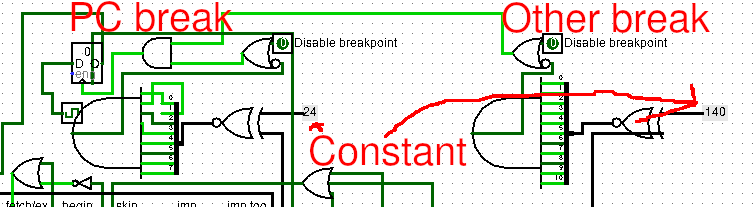
\includegraphics[width=\textwidth]{break.png}
		\caption{Set breakpoint\label{break}}
	\end{subfigure}
\end{figure}
\subsection{Loading program\label{Loading in}}
After you have written the program in assembly language, assembled it and debugged it in logisim it is time to load it in the minecraft computer. There is no way of doing this automaticly so you will have to plug in every instruction manually as described in section \ref{UI}. You can use the output file of your program to easily see the binary of every instruction.
\subsection{Example programs}
\subsubsection{Increment loop}
This is a very simple program that just infinitely increments the accumulator.
\begin{lstlisting}
var
one 0xfe 1

pgm
/infinite loop
loop	add one
	jmp loop
\end{lstlisting}
\subsubsection{Sorter\label{Round}}
The next program is a more complex program that sorts a list of values. These values must be between 0x600 (same as -512) and 0x1ff (same as 511). You can make the list of values anywhere in RAM. You define the position of the list by setting address 0xff (same as 255) and 0xfd (same as 253). In address 0xff you set the position of the first element of the list and and in address 0xfd you set the address of the last element of the list. You know that the program has finished running when the program counter constantly stays at the same address.

~\\
There are more efficient sorting algorithms than this one it is just an example. This program starts at the first item in the list where it will find the smallest value in the list and move that too the first item. Then it will go too the second item where it will find the second smallest value and so forth untill it hits the end of the list every time having to look for less and less values as it knows that the smaller values are already behind it.
\lstinputlisting{../sort}
In the lines 30-39 and 48-57 we can see the advantages of having a program stored in RAM. The program reads from and writes too a list. Every time it wants to read or write from a different element from this it changes the address of the instruction. This is something that can't be done in computers where the program is stored in ROM. An alternative way of accessing elements of lists is by using a stack, but this would add more complexity to the machine which is something I wanted to avoid.

%\lstinputlisting[firstline=1,lastline=19]{../sort}
%The program starts by copying the contents of the Beginlist address into i. The i address keeps track of the item in the list that it is currently searching a value for. The first value must be equal to the beginning of the list. It will then load the address of the end of the list and store it in the special variable NEndlist. This is done so the program doesn't have to negate Endlist all the time every time it wants to subtract and can just use NEnlist.

%\lstinputlisting[firstline=20,lastline=28]{../sort}\
%It checks if i variable has hit the end of the list. This it does by adding NEndlist with i and checking if the result is negative or not. If it isn't negative the program is finished and will jump to ``end" which is just an infinite loop, otherwise it will continue processing.

%\lstinputlisting[firstline=29,lastline=40]{../sort}
%This section of code really shows the advantages of having the program stored in RAM. When sorting the program often wants to read or write to the address specified by the i variable. To store to that address for example it load the value 0x100 into the accumulator and adds the contents of variable i to it. This it stores at the position of the instruction.

%\lstinputlisting[firstline=41, lastline=46]{../sort}
%It will now enter the second loop. In this loop it will compare every element that comes after the address specified in i with the value in the address specified by i. If ii is bigger than Endlist it means it has hit the end of the list and it will break loop2, increment i and go back to loop1.
\end{document}
